\documentclass[3p]{elsarticle} %review=doublespace preprint=single 5p=2 column
%%% Begin My package additions %%%%%%%%%%%%%%%%%%%

\usepackage[hyphens]{url}

  \journal{Scientific Data} % Sets Journal name

\usepackage{graphicx}
%%%%%%%%%%%%%%%% end my additions to header

\usepackage[T1]{fontenc}
\usepackage{lmodern}
\usepackage{amssymb,amsmath}
% TODO: Currently lineno needs to be loaded after amsmath because of conflict
% https://github.com/latex-lineno/lineno/issues/5
\usepackage{lineno} % add
  \linenumbers % turns line numbering on
\usepackage{ifxetex,ifluatex}
\usepackage{fixltx2e} % provides \textsubscript
% use upquote if available, for straight quotes in verbatim environments
\IfFileExists{upquote.sty}{\usepackage{upquote}}{}
\ifnum 0\ifxetex 1\fi\ifluatex 1\fi=0 % if pdftex
  \usepackage[utf8]{inputenc}
\else % if luatex or xelatex
  \usepackage{fontspec}
  \ifxetex
    \usepackage{xltxtra,xunicode}
  \fi
  \defaultfontfeatures{Mapping=tex-text,Scale=MatchLowercase}
  \newcommand{\euro}{€}
\fi
% use microtype if available
\IfFileExists{microtype.sty}{\usepackage{microtype}}{}
\usepackage[]{natbib}
\bibliographystyle{unsrt}

\ifxetex
  \usepackage[setpagesize=false, % page size defined by xetex
              unicode=false, % unicode breaks when used with xetex
              xetex]{hyperref}
\else
  \usepackage[unicode=true]{hyperref}
\fi
\hypersetup{breaklinks=true,
            bookmarks=true,
            pdfauthor={},
            pdftitle={Global multi-crop agricultural trial data supported by citizen science},
            colorlinks=false,
            urlcolor=blue,
            linkcolor=magenta,
            pdfborder={0 0 0}}

\setcounter{secnumdepth}{0}
% Pandoc toggle for numbering sections (defaults to be off)
\setcounter{secnumdepth}{0}


% tightlist command for lists without linebreak
\providecommand{\tightlist}{%
  \setlength{\itemsep}{0pt}\setlength{\parskip}{0pt}}




\usepackage{float}



\begin{document}


\begin{frontmatter}

  \title{Global multi-crop agricultural trial data supported by citizen
science}
    \author[a,b]{Kauê de Sousa%
  %
  }
   \ead{k.desousa@cgiar.org} 
    \author[a]{Marie-Angélique Laporte%
  %
  }
  
    \author[a]{Almendra Cremaschi%
  %
  }
  
      \affiliation[a]{
    organization={Bioversity
International},city={Montpellier},country={France},}
    \affiliation[b]{
    organization={University of Inland
Norway},city={Hamar},country={Norway},}
    \cortext[cor1]{Corresponding author}
  
  \begin{abstract}
  The triadic comparison of technologies (tricot) is a citizen science
  approach for testing technology options in their target environments,
  which has been applied to on-farm testing of crop varieties. `Triadic'
  refers to the sets of three technology options that are compared by
  each participant. In the approach, participants are invited to test a
  anonymous set of three technologies (out of a larger number, generally
  between 5 to 20) randomly assigned. Between 2011 and 2025 the tricot
  approach was applied in more than 25 countries across Africa, Asia,
  Europe and Latin America with more than 30 crops.
  \end{abstract}
    \begin{keyword}
    digital innovation \sep FAIR data \sep tricot approach \sep 
    participatory variety testing
  \end{keyword}
  
 \end{frontmatter}

According to \citep{deSousa2024} and \citep{vanEtten2019}

\begin{figure}[H]
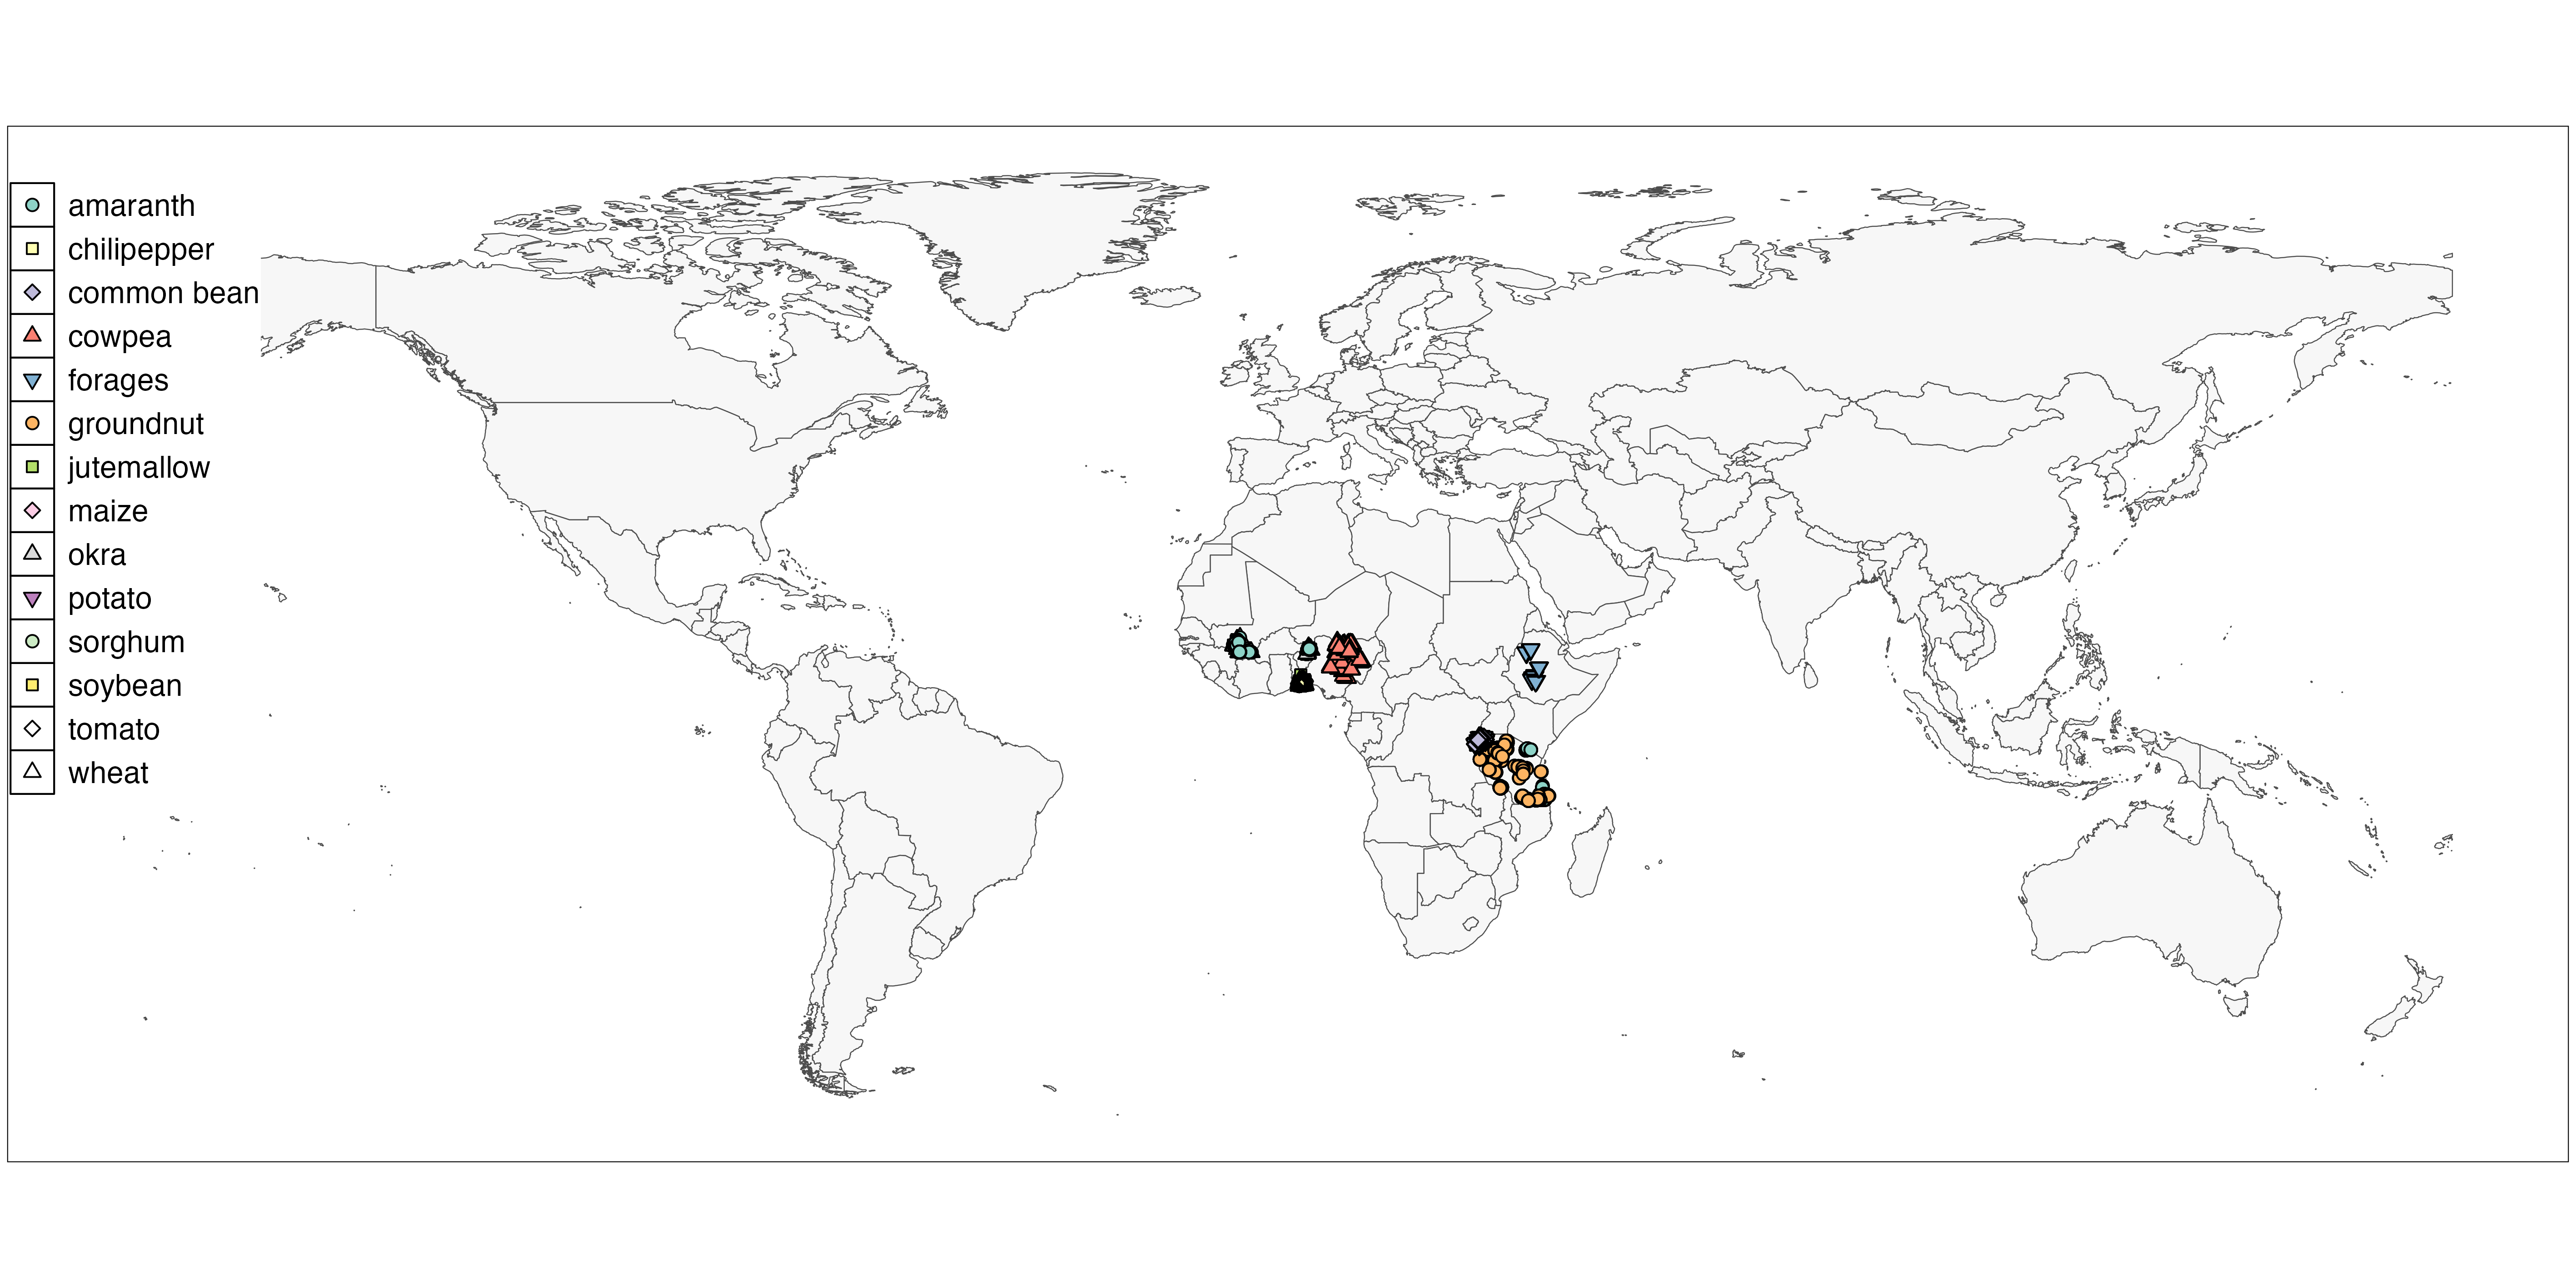
\includegraphics[width=1\linewidth]{trial-locations} \caption{Geographical distribution of crops and trial sites that are currently available for public use. Each point represents a trial location, and the legend indicates the crop(s) associated with those sites. Administrative boundaries are based on the Database of Global Administrative Areas (GADM). The authors remain neutral with regard to jurisdictional claims in maps.}\label{fig:map}
\end{figure}

\section{Acknowledgments}\label{acknowledgments}

This work has been supported by the projects 1000FARMS (INV-031561)
funded by the Gates Foundation, and BOLD Work Package 7 (Crop Trust Ref:
CONT-1522) funded by the Norwegian Agency for Development Cooperation
(Norad) through The Global Crop Diversity Trust.

\renewcommand\refname{References}
\bibliography{paper.bib}


\end{document}
